\documentclass[12pt, twoside]{article}
\usepackage[letterpaper, margin=1in, headsep=0.5in]{geometry}
\usepackage[english]{babel}
\usepackage[utf8]{inputenc}
\usepackage{amsmath}
\usepackage{amsfonts}
\usepackage{amssymb}
\usepackage{tikz}
\usepackage{yhmath}
%\usetikzlibrary{quotes, angles}

\usepackage{graphicx}
\usepackage{enumitem}
\usepackage{multicol}

\usepackage{fancyhdr}
\pagestyle{fancy}
\fancyhf{}
\renewcommand{\headrulewidth}{0pt} % disable the underline of the header

\fancyhead[RE]{\thepage}
\fancyhead[RO]{\thepage \\ Name: \hspace{3cm}}
\fancyhead[L]{BECA / Dr. Huson / 10th Grade Geometry\\* 16 May 2019}

\begin{document}
\subsubsection*{11.1 Do Now: Density \& compound shapes}
 \begin{enumerate}
  \item A lamp fixture is in the shape of a triangular pyramid. It is 7.2 inches tall and the area of its base is 11.5 in$^2$. Find the volume of the fixture to the \emph{nearest cubic inch}. \vspace{3cm}

  \item A marble statue has a volume of 1135 in$^3$. Find its weight, to the \emph{nearest tenth of a pound}. (assume the density of marble is 1.57 \emph{ounces} per cubic inch) \vspace{3cm}

  \item The area of the Bronx, NY is 42.47 square miles. Its population density is approximately 34,600 people per square mile. Estimate the population of the Bronx. \vspace{3cm}

  \item The volume of a cone is found to be 414.7 using the following formula:
    \[V=\frac{1}{3} \pi r^2 \times 11=414.7\]
    What does the value $11$ in the formula represent? Solve for the radius. \vspace{7cm}

\newpage
  \item BECA middle schoolers draw a basketball key on the asphalt in chalk. It is rectangular with one end round. It is 6 feet wide and overall it is 11 feet long, as shown. Find the area of the chalked basketball key to the \emph{nearest square foot}.\\[1.5cm]
    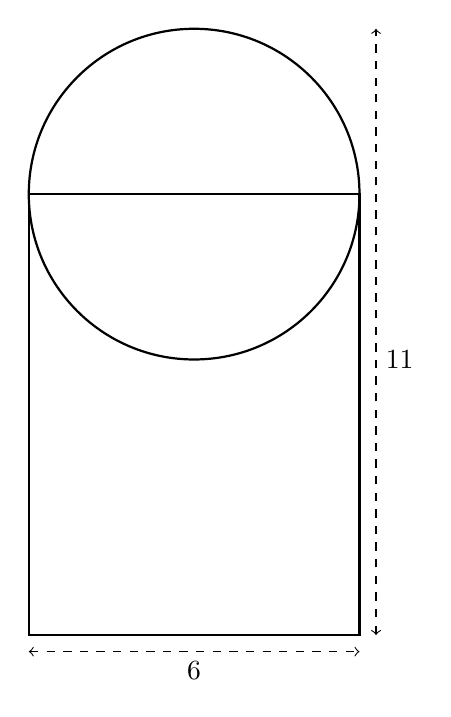
\begin{tikzpicture}[scale=0.7]
      \draw [thick]
      (0,0)--(0,8)--(6,8)--(6,0)--cycle;
      \draw [thick] (3,8) circle[radius=3];
      \draw [dashed,<->] (6.3,0)--(6.3,11);
      \draw [dashed,<->] (0,-0.3)--(6,-0.3);
      %\draw (0,8)++(0,-0.8)--++(0.8,0)--+(0,0.8);
      \node at (3,-0.3)[below]{$6$};
      \node at (6.3,5)[right]{$11$};
      %\node at (6.25,7)[right]{$2$};
    \end{tikzpicture}

  \item A wooden plank is laid on a brick platform. There are three steps leading to the platform, each 1 foot tall. The length of the plank is 16 feet. What is the angle of elevation, $x$, that the plank makes with the ground, to the \emph{nearest degree}.\\[1.cm]
        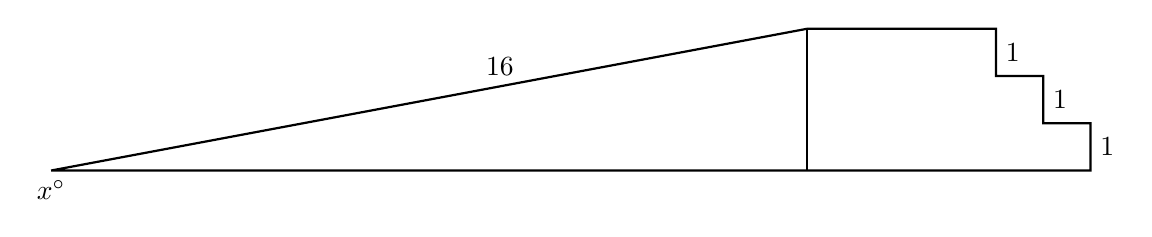
\begin{tikzpicture}[scale=0.6]
          \draw [thick] (-6,0)--(10,3)--(14,3)--(14,2)--(15,2)--(15,1)--(16,1)--(16,0)--cycle;
          \draw [thick] (10,0)--(10,3);
          %\draw (10,16)++(0,-0.8)--++(0.8,0)--+(0,0.8);
          \node at (16,0.5)[right]{$1$};
          \node at (15,1.5)[right]{$1$};
          \node at (14,2.5)[right]{$1$};
          \node at (-6,0)[below]{$x^\circ$};
          \node at (3.5, 1.8)[above]{$16$};
          %\node at (14, 4)[above]{\emph{Not to Scale}};
        \end{tikzpicture} \vspace{5cm}

  \end{enumerate}
  \newpage
  \setcounter{page}{1}
\subsubsection*{11.5 Pop Quiz: Density \& compound shapes}
 \begin{enumerate}

\item A candle has the shape of a cone. It is 8.5 inches tall and the diameter of its base is 4 inches. Find the volume of the candle to the \emph{nearest cubic inch}. \vspace{3cm}

\item A bronz trophy has a volume of 520 cm$^3$. Find its weight, to the \emph{nearest tenth of a kilogram}. (assume the density of bronz is $8.5 \ grams/ \mathrm{cm}^3$) \vspace{2.5cm}

\item The area of the Manhattan, NY is 22.82 square miles. Its population density is approximately 73,000 people per square mile. Estimate the population of Manhattan. \vspace{2.5cm}

\item The volume of a pyramid with a square base is found to be 245 using the formula:
  \[V=\frac{1}{3} x^2 \times 15=245\]
  What does the value $15$ in the formula represent? Solve for the length of the side of the square base. \vspace{7cm}

\newpage
\item Mott Hall fourth graders draw a basketball key on the asphalt in chalk. It is rectangular with one end round. It is 4 feet wide and overall it is 7 feet long, as shown. Find the area of the chalked basketball key to the \emph{nearest square foot}.\\[1.5cm]
  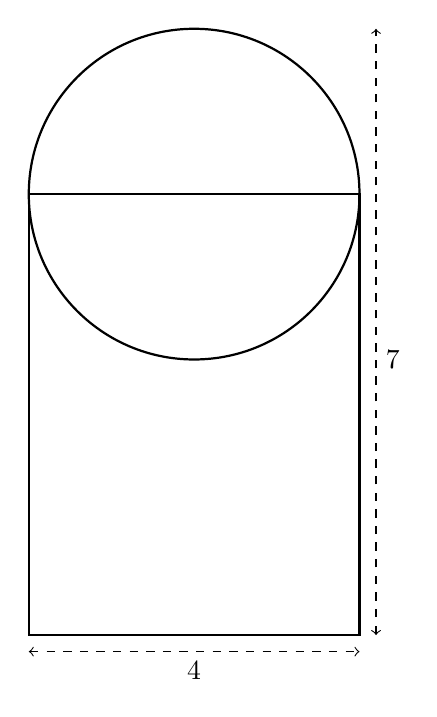
\begin{tikzpicture}[scale=0.7]
    \draw [thick]
    (0,0)--(0,8)--(6,8)--(6,0)--cycle;
    \draw [thick] (3,8) circle[radius=3];
    \draw [dashed,<->] (6.3,0)--(6.3,11);
    \draw [dashed,<->] (0,-0.3)--(6,-0.3);
    %\draw (0,8)++(0,-0.8)--++(0.8,0)--+(0,0.8);
    \node at (3,-0.3)[below]{$4$};
    \node at (6.3,5)[right]{$7$};
    %\node at (6.25,7)[right]{$2$};
  \end{tikzpicture}

\item A wooden plank is laid on a brick platform. There are two steps leading to the platform, each 1 foot tall. The length of the plank is 10 feet. What is the angle of elevation, $x$, that the plank makes with the ground, to the \emph{nearest degree}.\\[1.cm]
      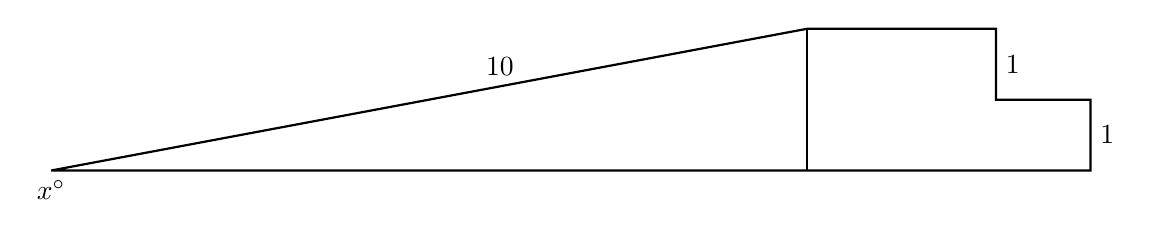
\begin{tikzpicture}[scale=0.6]
        \draw [thick] (-6,0)--(10,3)--(14,3)--(14,1.5)--(16,1.5)--(16,0)--cycle;
        \draw [thick] (10,0)--(10,3);
        %\draw (10,16)++(0,-0.8)--++(0.8,0)--+(0,0.8);
        \node at (16,0.75)[right]{$1$};
        \node at (14,2.25)[right]{$1$};
        \node at (-6,0)[below]{$x^\circ$};
        \node at (3.5, 1.8)[above]{$10$};
        %\node at (14, 4)[above]{\emph{Not to Scale}};
      \end{tikzpicture} \vspace{5cm}



  \end{enumerate}
  \newpage
  \setcounter{page}{1}
\subsubsection*{11.5 Homework: Volume, density, trig, \& compound shapes}
 \begin{enumerate}
  \item A cube has a volume of 670 cubic inches. What is the length of its side, to the \emph{nearest hundredth of an inch}? \vspace{3cm}

  \item The Great Pyramid of Giza was constructed as a regular pyramid with a square base. It was built with an approximate volume of 2,592,276 cubic meters and a height of 146.5 meters. What was the length of one side of its base, to the \emph{nearest meter}? \vspace{5cm}

  \item A bakery sells hollow chocolate spheres. The larger diameter of each sphere is 4 cm. The thickness of the chocolate of each sphere is 0.5 cm. Determine and state, to the \emph{nearest tenth of a cubic centimeter}, the amount of chocolate in each hollow sphere.\\[4.5cm]
  The bakery packages 8 of them into a box. If the density of the chocolate is 1.308 g/$\mathrm{cm}^3$, determine and state, to the nearest gram, the total mass of the chocolate in the box.


    \item A steel plate is shaped as a 6 inch square with a 2-inch tall triangle on one side, as shown. There are four circular holes in the plate, each having a 1 inch diameter. The plate is one quarter inch thick.
    \begin{enumerate}
      \item Determine and state the area taken up by the plate, subtracting the area of the holes, to the \emph{nearest tenth of a square inch}.\\[1.5cm]
        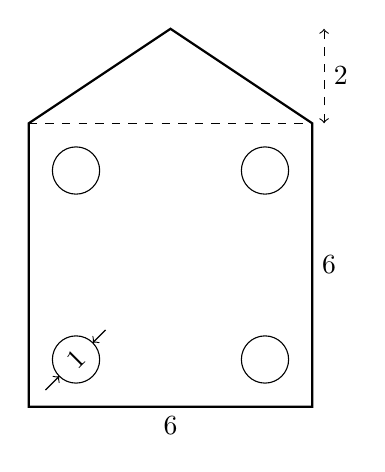
\begin{tikzpicture}[scale=0.6]
          \draw [thick]
          (0,0)--(0,6)--(3,8)--(6,6)--(6,0)--cycle;
          \draw [dashed] (0,6)--(6,6);
          \draw [dashed,<->] (6.25,6)--(6.25,8);
          \draw (1,1) circle[radius=0.5] node[rotate=45]{1};
          \draw [->] (45:0.5)--(45:0.9142);
          \draw [->] (45:2.3)--(45:1.9142);
          \draw (5,1) circle[radius=0.5];
          \draw (5,5) circle[radius=0.5];
          \draw (1,5) circle[radius=0.5];
          %\draw (0,8)++(0,-0.8)--++(0.8,0)--+(0,0.8);
          \node at (3,0)[below]{$6$};
          \node at (6,3)[right]{$6$};
          \node at (6.25,7)[right]{$2$};
        \end{tikzpicture} \vspace{1cm}
      \item Find the volume of the plate, to the \emph{nearest tenth of a cubic inch}. \vspace{2cm}
      \item Find the weight of the plate, to the \emph{nearest ounce}.
    \end{enumerate} \vspace{1.5cm}



\newpage
\item A concrete ramp with a $4^\circ$ angle of elevation leads to a platform with a staircase stepping down from the opposite side, as shown below. The length of the platform is 3 feet, and each of the four steps has a rise of 7 inches and run of 10 inches. Find the length of the ramp $x$, to the \emph{nearest inch}.\\[0.25cm]
      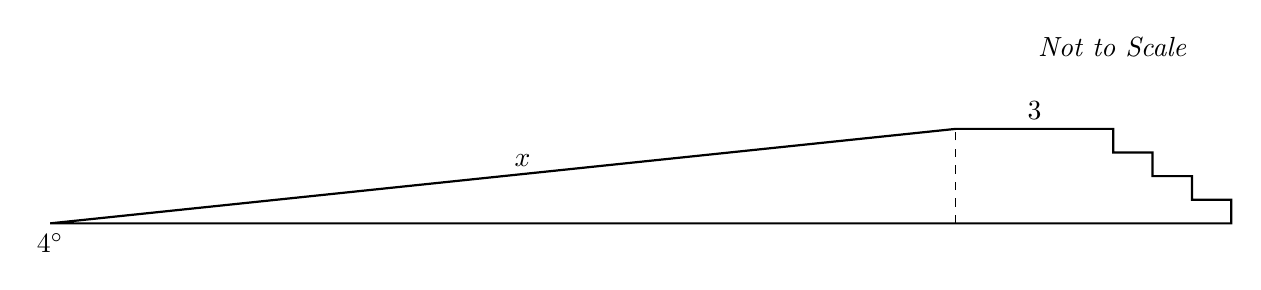
\begin{tikzpicture}[scale=0.5]
        \draw [thick] (7,0)--(30,2.4)--(34,2.4)--(34,1.8)--(35,1.8)--(35,1.2)--(36,1.2)--(36,0.6)--(37,0.6)--(37,0)--cycle;
        \draw [dashed] (30,0)--(30,2.4);
        %\draw (10,16)++(0,-0.8)--++(0.8,0)--+(0,0.8);
        \node at (32,2.4)[above]{$3$};
        \node at (7,0)[below]{$4^\circ$};
        \node at (19, 1.2)[above]{$x$};
        \node at (34, 4)[above]{\emph{Not to Scale}};
      \end{tikzpicture} \vspace{5cm}

\item A prescription medicine comes in capsule form. The capsule is in the shape of a cylinder with hemispherical ends, as shown in the rendering below. The capsule is 15 millimeters long by 8 millimeters across.
\begin{enumerate}
    \item Write down the radius $r$ of the capsule and the length of the cylindical portion $a$, shown in the diagram.\\
    \includegraphics[width=0.3\textwidth]{capsule.png}\\
    \item Find the volume of the capsule to the \emph{nearest cubic millimeter}.
  \end{enumerate}

\end{enumerate}
\end{document}
